\documentclass{article}[11pt]
\usepackage[frenchb,english]{babel}
\usepackage[T1]{fontenc}
\usepackage[utf8]{inputenc}
\usepackage{amsmath,amssymb,latexsym}
\usepackage{times}
\usepackage{float}
\usepackage[left=2cm,right=2cm,top=2cm,bottom=2cm]{geometry}
\frenchbsetup{StandardLists=true} % � inclure si on utilise \usepackage[french]{babel}
\usepackage{enumitem}
\usepackage{fancyhdr}
\usepackage{mathrsfs}
\usepackage{graphicx}
%\usepackage[Algorithme]{algorithm}
%\usepackage{algorithmic}
\usepackage{tikz}
\usepackage{tabularx}
\usetikzlibrary{shapes}
\pagestyle{fancy}
\newcommand{\tr}[1]{{\vphantom{#1}}^{\mathit t}{#1}} 
\renewcommand\headrulewidth{1pt}
\fancyhead[L]{Cours 1�re S}
\fancyhead[R]{Yoann Pietri}
\newcounter{theoremecounter}[subsection]
\usepackage{titlesec}
\setcounter{secnumdepth}{3}% enl�ve la num�rotation apr�s les sections
%\renewcommand\thechapter {\Roman{chapter}}

 \setlength{\parindent}{0pt}

\newcommand{\R}{\mathbb{R}}
\newcommand{\N}{\mathbb{N}}
\newcommand{\Q}{\mathbb{Q}}
\newcommand{\Z}{\mathbb{Z}}
\newcommand{\C}{\mathbb{C}}
\newcommand{\K}{\mathbb{K}}
\newcommand{\eqi}{\Leftrightarrow}
\titleformat{\subsubsection}
   {\normalfont\fontsize{11pt}{13pt}\selectfont\bfseries}% apparence commune au titre et au num�ro
   {\thesubsubsection}% apparence du num�ro
   {1em}% espacement num�ro/texte
   {}% apparence du titre

\tikzstyle{theobox} = [draw=black, very thick,
    rectangle, rounded corners, inner sep=10pt, inner ysep=20pt]
\tikzstyle{theotitle} =[fill=white, text=black,rounded corners,draw=black,very thick]

\fancyhead[L]{Contrôle chapitre 11}

\usepackage[c]{esvect}
\newcommand{\covec}[2]{\begin{pmatrix}#1 \\#2 \end{pmatrix}}

\begin{document}
\center
\Large Contrôle de cours
\flushleft
\center
Echantillonage
\flushleft \normalsize
Durée du contrôle : 1h\newline
Ce sujet comporte 3 pages\newline
La calculatrice est autorisée
\subsection*{Exercice 1 (R.O.C., temps conseillé : 10 min) : }
Rappeler le principe d'échantillonnage, ses objectifs et ce qu'il permet de faire. Dans le cas d'un échantillon de $n\geq 25$ personnes, le caractère $C$ apparaissant avec une proportion $0,2 \leq p \leq 0,8$, donner l'intervalle de fluctuation à 95\%
\subsection*{Exercice 2 (temps conseillé : 10 min) : }
On admet que dans la population française, le caractère "avoir le baccalauréat" est un caractère qui apparait avec une proportion $0,71$ (tous baccalauréats confondus). On tire au hasard 98 765 personnes dans la population française. Parmi ces personnes 69 234 personnes avaient un baccalauréat. Cet échantillon est-il représentatif de la population?
\subsection*{Exercice 3 (Algorithmique, temps conseillé : 20 min) : }
\begin{enumerate}
\item Ecrire un algorithme qui, à un entier $n$ saisi par l'utilisateur, renvoie le nombre $n!$. On admet qu'on peut l'utiliser dans les prochains algorithmes à l'aide de \begin{verbatim} factorielle(n) \end{verbatim}
\item Ecrire un algorithme qui, à deux entiers $n$ et $k$ saisis par l'utilisateur, renvoie le nombre $\binom{n}{k}$. On admet qu'on peut l'utiliser dans les prochains algorithmes à l'aide de \begin{verbatim} binom(k,n) \end{verbatim}
\item Ecrire un algorithme qui, à deux entiers $n$ et $k$ et à un nombre $p$ dans $[0,1]$ saisis par l'utilisateur, renvoie $P(X=k)$ où $X\sim \mathscr{B}(n,p)$. On admet qu'on peut l'utiliser dans les prochains algorithmes à l'aide de \begin{verbatim} PBinom(n,p,k) \end{verbatim}
\item Ecrire un algorithme qui, à deux entiers $n$ et $k$ et à un nombre $p$ dans $[0,1]$ saisis par l'utilisateur, renvoie $P(x\leq k)$ où $X \sim \mathscr{B}(n,p)$. On admet que l'on peut l'utiliser dans les prochains algorithmes par \begin{verbatim}PInfBinom(n,p,k)\end{verbatim}
\item Ecrire un algorithme qui, à un entier $n$ et à deux nombres $p$ et $p0$ dans $[0,1]$ saisis par l'utilisateur, renvoie le premier $k$ tel que $P(X \leq k) \geq p0$ où $X\sim \mathscr{B}(n,p)$. On admet que l'on peut l'utiliser dans les prochains algorithmes à l'aide de \begin{verbatim} LimSupBinom(n,p,p0) \end{verbatim}
\item Que représente \begin{verbatim} LimSupBinom(n,p,0.975) \end{verbatim} par rapport à l'échantillonage
\end{enumerate}
\subsection*{Exercice 4 (temps conseillé : 20 min) : }
On possède un paquet de carets contenant 3 cartes de coeur et 7 cartes de carreau. On tire 100 cents fois une carte dans ce paquet et on mélange entre chaque tirage. On note $X$ le nombre de cartes de coeur tirées
\begin{enumerate}
\item Quelle est la loi de $X$ ?
\item A l'aide des données issues d'un tableau, déterminer un intervalle de fluctuation au seuil de 95 \%
\center 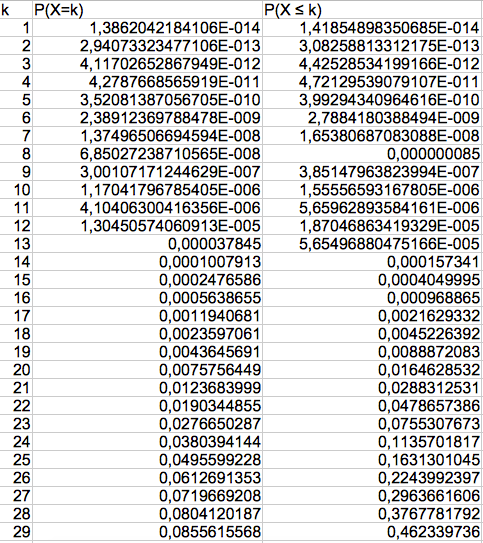
\includegraphics[scale=0.5]{chapp11_ill1.png} \flushleft
\center 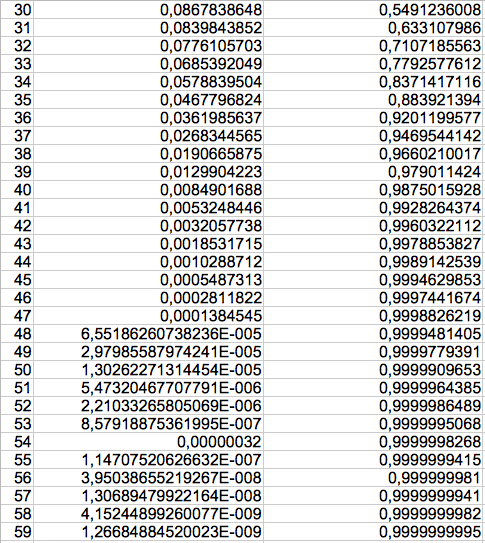
\includegraphics[scale=0.5]{chapp11_ill2.png} \flushleft
\center 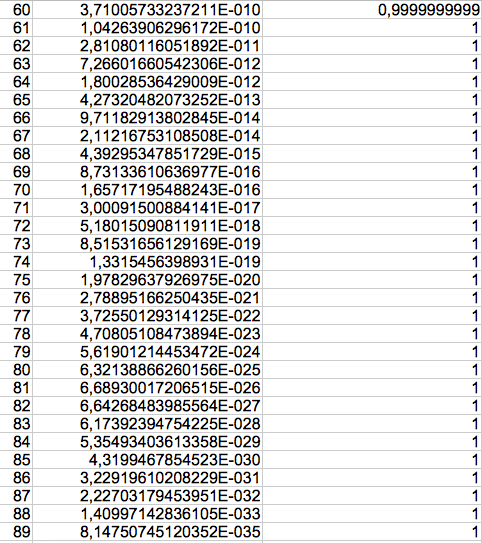
\includegraphics[scale=0.5]{chapp11_ill3.png} \flushleft
\center 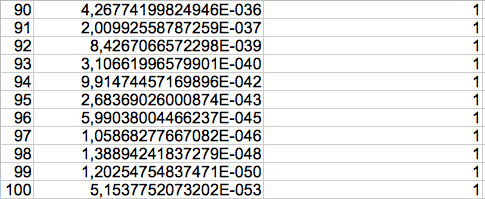
\includegraphics[scale=0.5]{chapp11_ill4.png} \flushleft
\item 3. Qu'aurait renvoyé 
\begin{verbatim} LimSupBinom(100,0.3,0.975) \end{verbatim}  ?
\item 4. Est ce que $P(x\leq k)$ est vraiment égal à 1 à partir de $k=61$. A quoi est dû ce phénomène ?
\item 5. Lors d'un essai, Max a tiré 41 cartes coeurs. Qu'en pensez vous ?
\end{enumerate}
$$\star \star \star$$
\center
FIN DU SUJET
\end{document}